\input{../../MiseEnPage/MiseEnPageParch'-1.3.tex}
\rhead{février 2015}

\let\newlist\relax		
\usepackage{enumitem}
\usepackage{calc}
\usepackage{textcomp}
\usepackage{aurical}

\DeclareSymbolFont{extraup}{U}{zavm}{m}{n}
\DeclareMathSymbol{\varheart}{\mathalpha}{extraup}{86}

\newcommand{\saintValentin}{{\hspace{\fill}$\varheart$\hspace*{3mm}}}

\usepackage{tikz}
\usepackage{pgfornament}
\usepackage{mathpazo}
\newcounter{row}
\newcounter{col}

\newcommand\setrow[9]{
  \setcounter{col}{1}
  \foreach \n in {#1, #2, #3, #4, #5, #6, #7, #8, #9} {
    \edef\x{\value{col} - 0.5}
    \edef\y{9.5 - \value{row}}
    \node[anchor=center] at (\x, \y) {\n};
    \stepcounter{col}
  }
  \stepcounter{row}
}

\newcommand\setrowgrand[9]{
  \setcounter{col}{1}
  \foreach \n in {#1, #2, #3, #4, #5, #6, #7, #8, #9} {
    \edef\x{\value{col} - 0.5}
    \edef\y{16.5 - \value{row}}
    \node[anchor=center] at (\x, \y) {\n};
    \stepcounter{col}
  }
}

\newcommand\setrowsuite[7]{
  \foreach \n in {#1, #2, #3, #4, #5, #6, #7} {
    \edef\x{\value{col} - 0.5}
    \edef\y{16.5 - \value{row}}
    \node[anchor=center] at (\x, \y) {\n};
    \stepcounter{col}
  }
  \stepcounter{row}
}

\begin{document}
\newgeometry{ignoreheadfoot,
	vcentering,
	hmargin=2cm,
	vmargin=3cm,
	bottom=1cm,
	footskip=.5cm	
	}

\thispagestyle{empty}
\vspace*{-2.5cm}{\centering\includegraphics[width=\textwidth]{../../images/logoParchEpure.png}}

\vspace*{-.7cm}\rule{0.87\textwidth}{1pt}\hspace{3pt}{février 2015}

\includegraphics[width=\textwidth]{images/couverture2gimpee1.png}

\includegraphics[width=\textwidth]{images/couverture2gimpee2.png}

\begin{center}
%\pgfornament[scale=.4, symmetry=h]{75}\\
{\Fontlukas{\fontsize{1.2cm}{1em}\selectfont Numéro spécial Saint-Valentin}}\\[2mm]
\pgfornament[scale=.4]{75}
\end{center}

\newpage
\restoregeometry


\vspace*{-1.9cm}
\begin{article}{L'Edito}
{Alicia Frésard}{QG de Charlie la licorne}

\begin{spacing}{.9}
\icsc{U}{n petit rayon} de soleil me nargue depuis un moment. Après le froid glacial de ce début d’année, serais-je dupe ? Qu’un moyen d’en avoir le cœur net : ni une ni deux, j’enfile ma grosse veste, des chaussettes, j’entrouvre la porte, pose un orteil au sol et… Au lieu de finir en glaçon, c’est une douce chaleur qui caresse mon pied. Enhardie, c’est sans plus réfléchir que je m’élance dehors, m’extraie de ma veste, remonte pantalon et t-shirt et profite de faire, enfin, le plein de lumière et de chaleur.

Une idée caresse mon esprit : prise de remords après cet hiver ni neigeux ni chaud (en somme pas terrible), la Terre voudrait-elle nous offrir un printemps précoce ? Mais oui, je le sens, le soleil s’installe de manière permanente cette fois-ci ! Fini les allers et venues météorologiques !

Cependant, le soir du 14 février, le ciel s’obscurcit : il faut compter sur la solidarité, corps contre corps, pour passer une chaude soirée. Les jours suivants sont terribles ! Moi qui rêvais déjà de sortir mes petites vestes et mes espadrilles, me revoilà engloutie sous un amas de couches de tissus à n’en plus finir !

Parfait ! Puisque l’on joue avec nos émotions, tâchons de garder le moral et d’attendre un peu plus longtemps ce printemps qui viendra, qui viendra… Et pourquoi ne pas profiter d’un Parchemin tout pensé en ce sens ? D’un Parchemin qui parle d’amour, d’écriture, de films, … 

Bon courage et bonne lecture !\\
A.F.
\end{spacing}
\end{article}


\vspace*{-2mm}\ligne\vspace*{-4mm}


\begin{article}
{Concours littéraire PIJA}
{Yitao et El Shaddai}{perdus dans les livres}

\begin{spacing}{.9}
\icsc{D}{e Staëliens}, de Staëliennes, à vos stylos, machines à écrire, ordinateurs... Bref, tout ce qui vous permet d'écrire librement! Le concours PIJA est de retour cette année, et le genre est à couper le souffle : la prose au sens large. Il n'y a pas de limites, pas de thème... En d'autres termes, vous êtes livrés à votre sens artistique et libres de faire comme vous le souhaitez !

\soustitre{Qu'est-ce que c'est ?}
Le PIJA (Prix Inter-régional des Jeunes Auteurs) est un concours qui a lieu chaque année qui permet à des jeunes auteurs comme vous et moi de confronter le public car les meilleurs textes seront publiés dans un recueil aux éditions de l'Hèbe. Il est basé à Charmey et implanté en Suisse Romande et n'importe qui de Franche-Comté, Vallée d'Aoste et Roumanie.

Cette année, le PIJA invite les jeunes à confronter la prose au sens large, tel que la nouvelle, le conte, la lettre, ou la prose poétique. Il n'y a aucun thème : l'originalité est clé!

\soustitre{Conditions de participation:}
\vspace*{-.8\baselineskip}\begin{itemize}[leftmargin=0cm,itemindent=.5cm]
	\item Être âgé de 15 à 20 ans le mardi 31 mars 2015
	\item Présenter un texte jamais publié, n’ayant bénéficié d’aucune récompense et n’excédant pas 10 pages dactylographiés ou 30'000 caractères (espaces compris).
	\item Autoriser la publication par les éditions de l’Hèbe
	\item Un(e) candidat(e) ne peut présenter qu’un texte par édition.
	\item Les textes collectifs ne seront pas pris en compte.
\end{itemize}\vspace*{.5\baselineskip}

\soustitre{Les prix:}
Qui dit concours, dit prix, et les éditions de l'Hèbe savent comment donner envie... Une somme de CHF 10'000.- (\texteuro 7'500.-) en espèces sera distribué entre les lauréats primés par le Jury international. Le premier prix peut attendre les CHF 2'000.- (€ 1'500.-).

Les textes retenus seront publiés dans un recueil dans les éditions de l'Hèbe, ce qui crée un lien, un nom, un début.

\soustitre{Les gagnants?}
Et les anciens gagnants ? Il n'y a rien de pire que de gagner un concours et se rendre compte, qu'au final, n'avoir rien gagner du tout ! Un ancien élève de notre cher collège vous dira bien le contraire... Joël Dicker a été nommé, par la Tribune de Genève, le plus jeune rédacteur en chef dans sa jeunesse, lorsqu'il fonda \textit{La Gazette des Animaux}. Mais son succès ne s'arrêta pas là, car en 2005 – comme vous l'avez bien deviné – sa nouvelle, \textit{Tigre}, attira l'attention du jury et lui gagna une place dans le recueil. Aujourd'hui, il est un auteur mondialement reconnu – avec un site internet et une page Wikipédia, oui oui – et son roman \textit{La Vérité sur l'affaire Harry Quebert} a fait fureur en français et se fait traduire en plusieurs langues, notamment l'anglais, en ce moment-même.\\
Plutôt pas mal, nan ?

\vspace*{-1mm}\includegraphics[width=\linewidth]{images/pija.png}\vspace*{-1mm}

\soustitre{Pour en savoir plus :}
Téléphone : +41269275030\\
Email : \url{conatact@pija.ch}\\
Site : \url{www.pija.ch}\\
Adresse : Editions de l'Hèbe SA, chemin du Lac 39, 1637 Charmey, CH
\end{spacing}
\end{article}




\newpage




\vspace*{-1.9cm}
\begin{article}
{Journée sportive}
{Les matelottes}{essoufflées après tant d'action}
\exerguedebutarticle[Sport]{Ce fut une journée pour le moins spéciale pour certain d'entre nous, un vendredi 30 intense en émotions, sports et raclette. Pour vous, un petit compte rendu des événements.}

\begin{spacing}{.94}
\icsc{A}{u petit matin}, dans le tram nous menant au collège, quelques personnes aux tenues surprenantes se distinguaient des autres. Des jeunes aux foulards dans les cheveux, aux chaussettes rose fluo, aux tenues sportives; des moustachus ou encore des licornes se dirigeaient vers de Staël. Le point commun de ces énergumènes? Leur corps athlétique ! La déduction qui suivait était donc simple, ça ne pouvait qu'être des troisièmes années ! Qui, accessoirement, se rendaient à leur journée sportive.

En effet, chaque degré a droit à sa petite récompense durant l'année. Les quatrièmes sont les plus chanceux avec leur voyage d'étude et leur journée neige qu'ils partagent avec les deuxièmes. Les premières et troisièmes se contentent d'une journée sportive. Mais autant vous dire que cette activité exceptionnelle est attendue avec impatience.

Enfin bref, revenons à notre récit.

Alors que vous suiez en cours de maths,  les troisièmes ont joué les grands sportifs. Entre ping-pong, streetball, badminton et volley, les athlètes n'avaient pas une minute de repos. C'est qu'ils devaient aussi prendre le temps d'aller encourager leurs amis, regarder le match de Stan, et bien sûr observer les corps de rêve qui s'acharnaient au jeu.

Aux alentours de midi, alors que vos estomacs commençaient à s'agiter, une très légère et délicieuse odeur s'est échappée de l'entrée du collège. Congelés autour d'une table à l'extérieur, les troisièmes se réchauffaient autour d'une traditionnelle raclette bien méritée, au vu des efforts sportifs faits. A noter que pour la première fois, la direction a fait preuve de grande rigueur en interdisant aux troisièmes de se réfugier à l'intérieur, ce qui vous aurait permis de profiter à plein nez de la bonne odeur !

Ayant repris de la forme grâce à ce sain repas, les troisièmes repartirent à la conquête de la victoire sportive. Et là, le drame. Alors que Wawrinka se battait avec succès contre Djoko, il perd lamentablement le dernier set et échappe à la victoire. Quelle déception ! Mais heureusement, au vu de la réussite sportive de ces troisièmes, la relève ne va pas tarder à arriver !

En fin d'après-midi, tous les meilleurs sportifs se sont retrouvés pour disputer leur dernier match, le match de leur vie, le match qui allait déterminer qui seraient les grands gagnants de chaque discipline. Vers 17h00 c'est le grand verdict! Les noms des gagnants ont eu l'honneur d'être inscrits sur... Une feuille!  Mais pas n'importe où attention... Sur le tableau d'affichage! (Ah non, pas celui dans le hall principal, près des salles de sport, faut pas exagérer non plus). Alors oui, ces vainqueurs sont rentrés les mains vides, mais la tête haute, le torse bombé, les t-shirts trempés et la fierté touchant à son paroxysme. Quelle gloire!

Les troisièmes ayant fait leur show, ce sera mardi au tour des quatrièmes et deuxièmes de nous montrer leurs prouesses à ski. Ne vous inquiétez pas, les aventures sportives du Collège de Staël ne sont donc pas finies!
\end{spacing}
\end{article}


\vspace*{-1mm}\ligne\vspace*{-4mm}


\begin{article}
{Des signatures qui font leur chemin\stamp{Votations}}
{Kita Enrire}{sans ses chaussettes mais à l'apogée du pouvoir}

\icsc{Ç}{a cogite} dans toutes les têtes et sous les stylos, bonjour ! En 2012, deux initiatives ont été lancées et ont récolté plus de 100'000 signatures pour enfin arriver au stade de votation populaire. Ah que d'humbles mots ! En effet, vous aurez jusqu'au 8 mars pour donner votre opinion, oui belles gentes, pour donner votre opinion et décider de votre avenir (enfin, là, vous avez une petite marge jusqu'au 30 avril concernant les futurs universitaires...). 

Permettez-moi un bref résumé : «Aider les familles, etc. », initiative déposée par le PDC, vise à déduire le montant des allocations familiales (versées pour chaque enfant) du revenu des parents. Ce montant, non-plus imposés soit décompté par les impôts, pourra donc être à l'entière disponibilité de la famille. En contrepartie, la Confédération verra une baisse de ses recettes et, selon elle, il ne serait pas exclu que les mesures d'économie dues à ces moindres recettes frappent également les familles (vous devinerez donc la position du conseil fédéral à ce sujet). 

« Taxer l’énergie », petit papier nous venant du Parti vert'libéral, souhaite quant à lui remplacer la TVA (taxe sur la valeur ajoutée) – que l'on observe normalement à la fin d'une facture et qui en augmente le montant – par une taxe sur les énergies non-renouvelables. De nouveau, la confédération tremble pour son argent, le pays des banques n'en mène pas plus large qu'un étudiant en période d'examens, se noyant dans le chocolat et retrouvant le goût de l'air frais. Mais justement, le rêve d'une Genève cycliste n'est peut-être plus si loin, reste à savoir si cette idée nous laisse un goût de miel ou de fuel dans la gorge...

\end{article}




\newpage





\vspace*{-1.7cm}\begin{article}
{FUN’raising débarque à de Staël}
{Ophélie C.}{en direct de l’UniGE}

\begin{spacing}{1.05}
\soustitre{L’alliance du divertissement et d’une cause humanitaire}
Tu souhaites défendre une cause humanitaire tout en passant du bon temps, mais tu ne sais pas à qui t’adresser? 
Tu souhaites changer le monde à ton échelle, mais tu n’as pas beaucoup de temps libre en parallèle de tes études ?
Tu te sens concerné(e) par les difficultés que rencontrent les enfants dans les pays défavorisés, mais tu ne sais pas comment apporter ta pierre à l’édifice?

Si tu as répondu OUI à au moins une de ces questions, alors FUN’raising est fait pour toi !

Mais qu’est-ce que FUN’raising au fait? FUN’raising est un projet caritatif visant à collecter des fonds afin de soutenir des associations connues pour leur engagement dans la lutte contre la misère et le travail des enfants. Comme son nom l’indique, ce projet allie divertissement et cause humanitaire.\columnbreak

\soustitre{FUN’pass : la clé du divertissement et de l’engagement}
Rien que pour vous, Staëliens, Staëliennes, FUN’raising met en place un calendrier d’activités diverses durant ce semestre. Pour participer aux activités, le FUN’pass est la clé. 

\exerguemilieuarticle{Amuse-toi et apporte ton soutien à des jeunes défavorisés}

Mais qu’est-ce que le FUN’pass au fait ? C’est votre passeport pour le divertissement engagé. Moyennant la modique somme de CHF 20, vous, étudiants, recevrez un pass crédité de 4 points, dont chacun vous permettra de participer à une activité et/ou d’acquérir un bon de tombola!\\
La tombola proposera des lots divers et variés, allant du séjour linguistique à l’étranger à une paire de lunettes Rayban !

Les enseignants sont invités à participer aux activités qui, par contre, leur coûteront chacune deux points.

\soustitre{Proposer une activité : Partage et découverte}
Staëliens, Staëliennes, comme vous l’aurez certainement compris, vous pourrez prendre part aux activités. Mais ce n’est pas tout ! Vous, étudiants comme enseignants,  aurez la possibilité d’organiser et d’animer une activité !\\
Partagez votre savoir ou votre passion avec les autres membres de l’établissement pour la bonne cause !

\soustitre{Qui contacter :}

\vspace*{-2\baselineskip}\begin{itemize}[leftmargin=0cm,itemindent=.5cm]
	\item \url{funraising2014@gmail.com}
	\item Madame Céline Zosso, enseignante d’Histoire et d’Anglais
	\item Liker la page Facebook FUN’raising (et partagez-la ! :D). Elle vous tiendra au courant des activités mises en place, de leurs lieux et leurs dates.
\end{itemize}
\end{spacing}
\end{article}



\ligne


\begin{article}
{Les JEC, c'est chouette\stamp{festival}}
{Otra}{sur son siège de cinéma}
\exerguedebutarticle[Cinéma, culture]{Les Journées d’Etude Cinématographique, c'est quoi ? Petite présentation de 3 journées plutôt sympas ! }

\begin{spacing}{1.06}
\icsc{V}{ous êtes amateurs} de cinéma ? Vous voulez passer 3 jours complets à regarder des films à la place d’aller en cours ET être excusés par la direction ? Peut-être même rencontrer l’amour dans l’intimité des salles sombres de cinéma ? Les Journées d’Etude Cinématographique (aussi appelées JEC par les intimes) sont faites pour vous ! Chaque année, le Grütli ouvre ses portes aux étudiants du post obligatoire pour accueillir ces fameuses JEC et nous propose de découvrir le travail d’un réalisateur. Au rythme de 2 films par jours, suivis généralement d’une heure de discussion en groupes réduits, ces journées offrent un beau survol de l’œuvre dudit réalisateur (enfin, pour ceux qui ne s’endorment pas…oui oui je vous ai vus petits coquins !).

Celles de 2015 sont malheureusement déjà finies, et ce sont les films de Roman Polanski qui ont été mis à l’honneur cette année. Pour les intéressés, gardez en tête l’existence de ces journées et repérez les affiches qui apparaissent généralement aux alentours de décembre (les JEC se déroulent en février) ! Les places sont limitées mais si vous n’êtes pas de la partie une année, retentez l’année suivante ! En espérant toutefois qu’elles survivent aux fameuses coupes budgétaires de l’Etat, puisqu’elles sont chaque année menacées de disparition. Alors continuez à soutenir ces magnifiques journées, parce qu’elles le valent bien !
\end{spacing}
\end{article}


\newpage
\newgeometry{ignoreheadfoot,
	vcentering,
	hmargin=2cm,
	vmargin=3cm,
	bottom=2cm,
	footskip=.5cm	
	}

\vspace*{-1.9cm}\begin{article}
{The imitation game \stamp{cinema}}
{Bebert et Xou}{au calme, posey dans le ciney}

\begin{spacing}{.9}
\icsc{A}{h, la St-Valentin}, quelle belle fête, vraiment! Les amoureux se déclarent leur flammes, les couples en profitent pour passer une soirée inoubliable, les romantiques écrivent des poèmes... Par contre, pour tous les autres, la St-Valentin consiste en une chouette journée de déprime et d'auto-apitoiement  sur le fait que – comme vous avez dû le dire au dernier repas de famille – <<je suis pas en coupleeeuh>>. 

Du coup, quitte à déprimer, autant le faire devant un film.\\
« The imitation game » ( à dire « le jeu de l'imitation » pour les guignes en anglais ) est un biopic sur la vie du malheureusement méconnu Alan Turing, père de l'informatique.\\
Le film, bien que plutôt académique, se révèle sympathique et bourré d'informations sur la deuxième guerre mondiale. De plus, les fanatiques de Sherlock pourront admirer leur acteur fétiche – j'ai nommé Benedict Cumberbatch – interpréter à merveille le rôle principal. Bien évidemment, les connaisseurs râleront un brin quant au côté romancé de l'histoire, mais avec le grand méchant  Hollywood aux commandes, il ne fallait pas rêver, d'autant que l'histoire telle qu'elle est racontée est vraiment touchante ( attention : risque d'yeux rougis à la fin de la séance ). Donc si en ce triste mois de février une envie subite de vous cultiver vous prenait ( si, si, ça arrive ), je ne peux que vous conseiller « The imitation game ». En plus, avec un peu de chance, vous arriverez peut-être à quelque chose en y invitant votre dulcinée.
\end{spacing}
\end{article}

\vspace*{-5mm}
\begin{center}
{\pgfornament[scale=.5, ydelta=-2mm]{72}\hspace*{2mm}
{\fontsize{1cm}{1em}\selectfont{\Fontlukas Dossier Saint-Valentin}}}
\hspace*{2mm}\pgfornament[scale=.5, ydelta=-2mm]{73}
\end{center}
\vspace*{-3mm}

\encadre[.97]{Quel amoureux es-tu?\saintValentin}{
\vspace*{0mm}
\begin{multicols}{3}
\begin{enumerate}[leftmargin=0cm,itemindent=.5cm, itemsep=0mm]
	\item Ta matière préférée :
	\begin{itemize}[itemindent=.3cm, topsep=-4pt, itemsep=-2mm]
		\item[$\star$]Les maths.
		\item[$\bullet$]Le français.
		\item[\tiny{$\blacksquare$}]L'éducation physique.
	\end{itemize}
	\item Où lis-tu généralement le Parchemin ?
	\begin{itemize}[itemindent=.3cm, topsep=-4pt, itemsep=-2mm]
		\item[\tiny{$\blacksquare$}]Dans les couloirs ou dans le hall.
		\item[$\bullet$]En classe.
		\item[$\star$]Chez toi.
	\end{itemize}
	
	\item Tu préfères t'endormir :
	\begin{itemize}[itemindent=.3cm, topsep=-4pt]
	\setlength\itemsep{-2mm}
		\item[$\bullet$]Sur le côté.
		\item[$\star$]Sur le dos.
		\item[\tiny{$\blacksquare$}]Sur le ventre.
	\end{itemize}
	
	\item Tes couleurs préférées :
	\begin{itemize}[itemindent=.3cm, topsep=-4pt]
	\setlength\itemsep{-2mm}
		\item[\tiny{$\blacksquare$}]Orange ou jaune.
		\item[$\star$]Vert ou bleu.
		\item[$\bullet$]Rouge ou violet
	\end{itemize}
	
	\item Tu préfères manger :
	\begin{itemize}[itemindent=.3cm, topsep=-4pt]
	\setlength\itemsep{-2mm}
		\item[$\star$]Simplement fait maison.
		\item[\tiny{$\blacksquare$}]Sur le pouce.
		\item[$\bullet$]Gastronomique.
	\end{itemize}
	
	\item La rubrique du Parch' que t'aimes le plus :
	\begin{itemize}[itemindent=.3cm, topsep=-4pt]
	\setlength\itemsep{-2mm}
		\item[$\bullet$]L'interview du prof.
		\item[\tiny{$\blacksquare$}]Les jeux !
		\item[$\star$]L'actu.
	\end{itemize}
\end{enumerate}

\columnbreak
\textbf{Tu obtiens une majorité de {\tiny{$\blacksquare$}}: Le Serial Lover}\\
Profiter, s'amuser, savourer : Voilà les mots qui te régissent ! Tu distingues clairement ami-e-s et petit-e ami-e. Sûr-e de ton charme, tu es direct-e. Pour toi, la relation amoureuse ne doit pas tenir artificiellement, si on ne s'entend plus, on ne va pas se mentir, c'est fini entre nous ! Mais comme tu ne veux pas rester seul-e, tu cherches à te caser au plus vite… Ok, mais il ne faut peut-être pas trop collectionner, au risque de devenir un "Casanova" ! 

\textbf{Tu obtiens une majorité de $\bullet$: Le Romantique}\\
Tu es un-e romantique transi-e. Les poèmes et les fleurs sont tes alliés dans la recherche de l'âme sœur. A l'inverse des Platoniques solitaires et des "Casanova", tu situes tes sentiments entre la tête et l'entrejambe, dans la partie émotive de ton corps : le cœur. Tu recherches avant tout la sincérité et une relation stable. Ça risque d'être long, mais tu as les poèmes et les fleurs comme alliés dans ta quête de l'âme sœur!

\textbf{Tu obtiens une majorité de $\star$: Le Platonique}\\
Les relations amoureuses ne t'intéressent pas particulièrement. Tu n’es ni prude, ni hostile à l’amour ; ce n’est simplement pas ta priorité. Tu considères ce type de relation comme futile et superflu, et as tendance à privilégier l’amitié. Tu es quelqu’un de rationnel : tu réfléchis beaucoup, parfois trop, et accordes une attention particulière aux qualités intellectuelles de ceux qui t'entourent. Ton esprit sérieux et méthodique fait de toi une personne réticente à s’engager, mais en bon philosophe que tu es, tu auras la patience nécessaire pour trouver la personne qui te conviendra !
\end{multicols}}




\newpage




\vspace*{-1cm}
\begin{article*}
{À ceux qui ont toujours voulu le faire\saintValentin}
{Poub' et Anton Nomase}{à l'église}

\begin{spacing}{.98}
\icsc{M}{ais qui} n'a jamais rêvé de le faire autre part qu'au lit ? Toi, par exemple, n'as-tu jamais ressenti l'excitation grisante de se retrouver dans pareille situation, l'angoisse constante de se faire attraper, d'envers et contre tout, assouvir le besoin bestial et primitif qui anime tout un chacun ? Oui, aujourd'hui, au temps de la grenouillère Winnie l'Ourson et de l'esclavagisme des concombres de mer gris, nous allons te libérer de l'hégémonie exercée par la société ! Oui, aujourd'hui est un grand jour, car une ère nouvelle va s'ouvrir à toi. Ô Collégien, il est temps de t'ériger vers des strates de plaisirs insoupçonnées ! Grâce à nous, ta vie va changer !
Par l'entremise de nos conseils avisés, nous allons t'offrir la possibilité de transcender un misérable, vulgaire, pathétique cours de maths en un instant sensuel, en solo ou à plusieurs (eh oui, au Parchemin, on apprécie à sa juste valeur l'ancestral art mathématique).

Pour commencer notre voyage au pays des merveilles (attention ça glisse !), découvrons comment le faire dans sa manière la plus basique. Pour ce faire, il vous faut : une chaise, un bureau bien solide, et, au besoin, une gomme, un crayon, une trousse ou, pour ceux que la taille n'effraie pas, un classeur. Nous allons vous présenter trois positions originales et source de fortes sensations. Bien évidemment, les rédacteurs du Parch' se sont fait un plaisir de les essayer. Force est de constater leur efficacité.

Le manche à trois doigts : (en solo) cette position vous donnera un maximum de plaisir pour un minimum de visibilité. Placez le membre de votre choix sur la surface dure du bureau, choisissez avec doigté la partie de votre corps qui va tenir bon aux à-coups. De plus, soyez prêt à opérer sur ce dernier une torsion d'au moins nonante degrés, si vous voulez en retirer quelque plaisir. Disposez harmonieusement votre tête sur le membre de votre choix. Pour un rendu optimal, ancrez votre membre à votre tête, au moyen de trois points, que l'on nommera G, G' et G''. Ainsi, vous pouvez le faire en toute quiétude, sans craindre de vous faire attraper.

\exerguemilieuarticle{<<Vous en avez marre de la routine ? Vous voulez le faire dans des endroits incongrus ? En classe !? Dans cet article, vous trouverez tout ce dont vous avez besoin pour assouvir ce désir.>>}

L'éléphant à grande trompe: (en solo, mais plaisir partagé) Commencez par imprimer une légère poussée arrière sur votre séant, de sorte que votre membre ait la place nécessaire pour s'étendre et exprimer son plein potentiel. Si vous possédez la souplesse nécessaire courbez votre dos exposant ainsi votre centre nerveux à toutes les sensations. Pour finaliser la position placer votre tête dans le creux de votre membre au point de friction entre une mollesse confortable et une érection turgescente. Une vague de chaleur vous aidera à atteindre le paroxysme du bien-être en société. Afin de partager votre plaisir avec votre voisin, vous pouvez laisser l’extrémité du membre se déposer sur le haut de son occiput et tracer des mouvements circulaires sur sa partie touffue.

Le nid du serpent: (à deux ou plus) L’entrelacement de vos membres respectifs donnera à cet acte une tendresse assurée. Pour plus de sécurité, il est recommandé d'utiliser deux bureaux jumeaux, mais distincts. Allongez votre torse musclé ou votre poitrine plantureuse sur un bureau et croisez vos membres avec ceux de votre voisin. Finissez par poser votre tête sur ce savant entrelacs et savourez cette petite pause à deux.

 Vous avez à présent connaissance de trois manières différentes pour pouvoir tranquillement dormir en classe. Quoi ? Ce petit pronom ne sous-entendait-il pas autre chose que le simple fait de fermer quelques instants les yeux de manière hautement philosophique durant une envolée lyrique mathématique ? Eh bien oui, uniquement cela. En moyenne un être humain passe trente ans dans son lit. Nous trouvons ces chiffres absolument affligeants. Si vous suivez nos méthodes à la lettre, nous vous garantissons cinquante-cinq virgule quarante-trois années de sommeil ! Au minimum !

\textit{Note de l'agence en relation de communication : Au vu des nombreuses plaintes d'étudiants en échec ayant appliqué rigoureusement les méthodes de cet article, la rédaction précise qu'elle n'est absolument pas garante des conséquences que pourrait avoir l'augmentation du nombre d'heures de sommeil sur les résultats scolaires desdits étudiants.}

\vspace*{9mm}\encadre{Mmm, lave-moi encore...!}{Pour certaines personnes, il est absolument hors de question qu'on s'approche d'un iota de leurs oreilles. Pour d'autres, l'inverse se produit : c'est un kiff complet, l'orgasme assuré. Histoires de métabolismes défaillants ? Que nenni : en effet, le conduit auditif externe peut se révéler être une puissante zone érogène. A l'instar de tout orifice corporel, la sensibilité y est accrue... Majoritairement préservée de contact et richement fournie en nerfs, cette zone en devient terriblement sensible.\\
Alors messieurs, mesdames : tous à vos coton-tiges !

Source: Néon Jan. 15}
\end{spacing}
\end{article*}




\newpage




\vspace*{-1.9cm}\begin{article}
{Playlist de la Saint-Valentin\saintValentin}
{Le musicien}{salle de musique}

\begin{spacing}{.9}
\icsc{Q}{ue serait} la Saint-Valentin sans musique? Cette année, le parchemin vous propose une playlist Rock! 

C'est bien connu, les groupes de Hard Rock et metal font les meilleures balades! On commence notre exploration des grands classique avec Elvis Presley et sa fameuse chanson "Let me Be Your Teddy Bear". On passe par les années 70/80, avec le groupe  Van Halen, et leurs titres "Why Can't This Be Love" et Can't Stop Lovin' You", idéals pour ce jour. On continue avec Scorpions et son légendaire "Still Loving You", classique indémodable. N'oublions pas les ZZ Top, avec leurs tubes mémorables comme "I need You Tonight" et "Gimme All Your Lovin'". On poursuit notre exploration de la musique des années 80-90 avec quelques groupes phares, comme Guns N' Roses, "Sweet Child O' mine", AC/DC "You shook Me All Night Long", puis on revient progressivement en passant par les années 2000, avec des groupes un peu plus violents pour certains, tel Rammstein, "Stirb Nicht Vor Mir (Don't Die Before I Do)", "Amour" et Slipknot (oui, ce groupe a des chansons parlant d'amour. Si si, allez écouter!) "Snuff", "The Nameless" (faites gaffe, cela reste du Nu Metal). Et pour bien finir en beauté, "I'm' a Believer" de Smash Mouth, reprise dans Shrek notamment.

Sur ce, bonne écoute!
\end{spacing}
\end{article}


\vspace*{-2mm}\ligne\vspace*{-4mm}\begin{article}
{<<Hé, mademoiselle...>>\saintValentin}
{Matthis E. Pasche \& Aline Mo}{connexion neuronale}
\exerguedebutarticle[Astuce drague]{Draguer, d'accord, mais au collège, on se doit de draguer avec intelligence. Ou plus exactement en étalant son savoir...}

\begin{spacing}{.9}
\icsc{L}{a Saint-Valentin}, la romance, l'amûûûr, c'est bien joli… Mais soyons honnêtes, et regardons la réalité en face: notre ère est celle de la drague. Messieurs, vous qui sifflez les demoiselles à tout bout de champ et qui creusez vos petites têtes à la recherche de la meilleure entrée en matière, nous sommes là pour vous rappeler que vous êtes au collège, ce puits de savoir (mais si, mais si). Ainsi donc, puisqu'il paraît que vous faites partie de l'élite intellectuelle, pourquoi ne pas en profiter pour étaler un peu votre science? Ça fait toujours du bien, et ça ne peut en tout cas pas vous rapporter moins de succès que des «hé, mademoiselle, t'es mignonne, tu me donnes ton numéro de téléphone?».

Amoureux de la littérature ancienne et moderne, vous pouvez bien sûr déclamer les vers ou la prose qui vous plairont, mais nous vous recommandons particulièrement le litotique <<Va, je ne te hais point!>> de Corneille. Assurez-lui qu'entre vous, il n'y aura pas de rejets, seulement des enjambements. Remontez le temps au-delà de la Rome antique, et trouvez-lui des épithètes dignes d'Homère,\columnbreak telles que Circé à la belle chevelure ou Aurore aux doigts de rose -- conseil: évitez peut-être Héra aux yeux de bœuf, pas le top niveau séduction. Et enfin, n'ayez pas peur d'être directs, tant que c'est avec savoir; offrez-lui de voir votre anapeste...


Du côté des atomes crochus, les possibilités sont nombreuses aussi. Faites-lui remarquer les flux d'ocytocine et de phényléthylamine qui circulent entre vous, et, en lui offrant un bouquet d'angiospermes:\\
(chimique) «Voudriez-vous que l'on crée une liaison covalente ensemble?»\\
(mathématique) «Quelle est la fonction qui vous dessine des courbes aussi parfaites?»\\
(physique) «Si Newton nous avait
\includegraphics[width=.64\textwidth]{images/coeurFonction.jpg}\columnbreak

vus, nul doute qu'il aurait aussitôt trouvé la loi d'attirance des corps!»
(géométrique) «Êtes-vous approximativement égale à 1,6180339887? Parce que vous êtes une fille en or!»

Oubliez les lettres d'amour, une simple équation suffit: $(x^2 + y^2 - 1)^3 - x^2y^3 = 0$, et le tour est joué! Et surtout, ne soyez pas trop sévère, laissez-la avoir peur des araignées et des serpents -- tant qu'elle n'est pas ithyphallophobe...

Et si les choses sont vraiment sérieuses entre vous, passez à l'étape supérieure; si vous avez dix-huit ans révolus et êtes tous deux capables de discernement, intéressez-vous à l'article 94 du Code civil suisse!
\end{spacing}
\end{article}




\newpage



\vspace*{-1.8cm}\titre{Mots-croisés}
\vspace*{-5mm}\begin{minipage}{.48\textwidth}
\tikzstyle {gridstyle}=[thick]
\begin{tikzpicture}[scale=1.32, every node/.style={scale=1.32}]
\hspace{-4mm}
\begin{crossgrid}[h=12,v=12]
\blackcases{1/1, 1/3, 1/7, 2/6, 2/9, 2/11, 3/7, 4/3, 4/8, 5/6, 5/9, 6/2, 6/5, 6/9, 7/8, 7/12, 8/4, 8/7, 8/10, 9/2, 9/6, 9/11, 10/4, 10/8, 11/1, 11/11, 12/8, 12/12} \end{crossgrid}
\end{tikzpicture}
\end{minipage}\hspace*{5mm}\begin{minipage}{.48\textwidth}
\textbf{Horizontal}
\vspace*{-2mm}\begin{multicols*}{2}
\maDef{h}{Poignée d'amour}\\
\maDef{h}{Tenu par un fil / gloussé / retira}\\
\maDef{h}{Symbole du sodium / recroquevillées dans un lieu chaud et réconfortant}\\
\maDef{h}{Péripatéticiennes / policier nazi}\\
\maDef{h}{Impudiques/ convia}\\
\maDef{h}{Petit nom des cartes mémoire / homme sous l'influence de Sirius / Services Industriels Genevois}\\

\columnbreak

\maDef{h}{Jardin paradisiaque / Sous espèce}
\maDef{h}{Accessoire de Cupidon / pécho / à deux}\\
\maDef{h}{Young Boy / On peut se la dorer ou l'avaler}\\
\maDef{h}{Relatif aux tripes / Excalibur, Durandal}\\
\maDef{h}{Érotique}\\
\maDef{h}{Femme qui nie / riche}\end{multicols*}
\end{minipage}

\vspace*{-2mm}\textbf{Vertical}
\vspace*{-3mm}\begin{multicols}{4}\setcounter{cntdef}{0}
\maDef{v}{Genre musical / Chipmunks crâneur}\\
\maDef{v}{Bon latin /métal qui  crée la ruée}\\
\maDef{v}{Cotons doux / de l’eau ou d’orientation}\\
\maDef{v}{United States / Inséparable la lyre / joli}\\
\maDef{v}{Escarboucle / préposition de provenance / Flux internet d’information}\\
\maDef{v}{Logarithme naturel / passion intense, brûlante / balle de service gagnante}\\
\maDef{v}{Rongement / ondulation d’un tissu}\\
\maDef{v}{Pieu / dévêtu / ...-joint / quatrième note de la gamme naturelle}\\
\maDef{v}{Dernière lettre de l’alphabet hébreu / l’acteur en joue}\\
\maDef{v}{Pour moi et pour... / ...belle a les yeux bleus, les yeux bleus ...belle a / Arbre de Malaisie qui produit du latex toxique}\\
\maDef{v}{Bourse à spermatozoïdes}\\
\maDef{v}{Frottement thérapeutique / Abréviation de couronne estonienne}\\
\end{multicols}

\ligne
\vspace*{-3mm}
\titre{Sudokus}\vspace*{1mm}
\begin{minipage}{.48\textwidth}
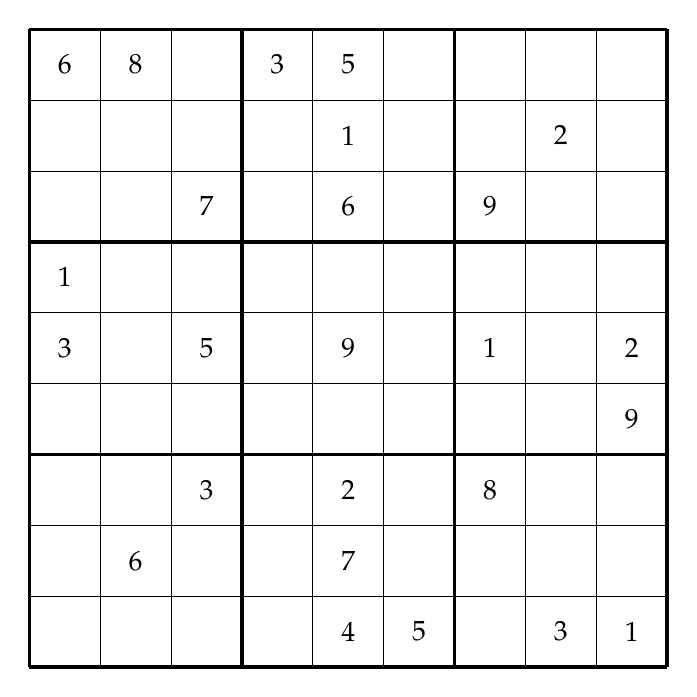
\begin{tikzpicture}[scale=.9]
\draw (0, 0) grid (9, 9);
    \draw[very thick, scale=3] (0, 0) grid (3, 3);

    \setcounter{row}{1}
    \setrow {6}{8}{ }  {3}{5}{ }  { }{ }{ }
    \setrow { }{ }{ }  { }{1}{ }  { }{2}{ }
    \setrow { }{ }{7}  { }{6}{ }  {9}{ }{ }

    \setrow {1}{ }{ }  { }{ }{ }  { }{ }{ }
    \setrow {3}{ }{5}  { }{9}{ }  {1}{ }{2}
    \setrow { }{ }{ }  { }{ }{ }  { }{ }{9}

    \setrow { }{ }{3}  { }{2}{ }  {8}{ }{ }
    \setrow { }{6}{ }  { }{7}{ }  { }{ }{ }
    \setrow { }{ }{ }  { }{4}{5}  { }{3}{1}
\end{tikzpicture}
\end{minipage}\hspace*{7mm}\begin{minipage}{.48\textwidth}
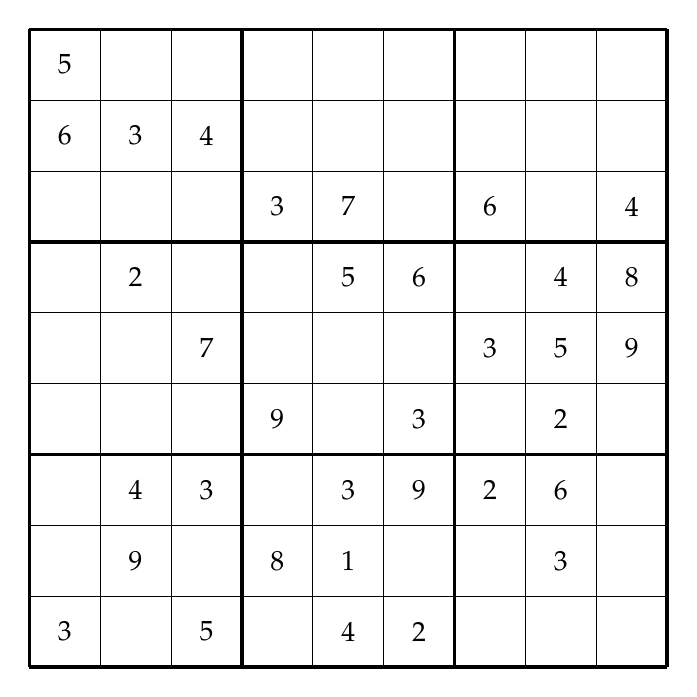
\begin{tikzpicture}[scale=.9]
\draw (0, 0) grid (9, 9);
    \draw[very thick, scale=3] (0, 0) grid (3, 3);

    \setcounter{row}{1}
    \setrow {5}{ }{ }  { }{ }{ }  { }{ }{ }
    \setrow {6}{3}{4}  { }{ }{ }  { }{ }{ }
    \setrow { }{ }{ }  {3}{7}{ }  {6}{ }{4}

    \setrow { }{2}{ }  { }{5}{6}  { }{4}{8}
    \setrow { }{ }{7}  { }{ }{ }  {3}{5}{9}
    \setrow { }{ }{ }  {9}{ }{3}  { }{2}{ }

    \setrow { }{4}{3}  { }{3}{9}  {2}{6}{ }
    \setrow { }{9}{ }  {8}{1}{ }  { }{3}{ }
    \setrow {3}{ }{5}  { }{4}{2}  { }{ }{ }
\end{tikzpicture}
\end{minipage}

\end{document}